\documentclass[tikz,border=4pt]{standalone}
\usepackage{amsmath,amssymb}
\usetikzlibrary{arrows.meta}

\begin{document}
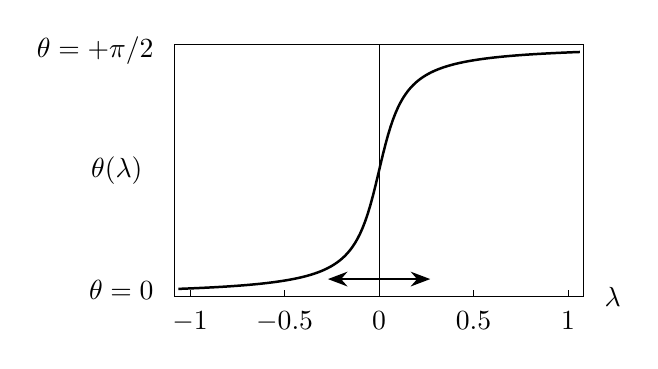
\begin{tikzpicture}[
  >=Stealth,
  font=\normalsize,
  axis/.style={line width=0.4pt},
  curve/.style={line width=0.9pt}
]
  % Box frame: lambda in [-1, 1] -> x in [-2.6, 2.6], theta in [0, pi/2] -> y in [0, 3.2]
  \draw[axis] (-2.6,0) rectangle (2.6,3.2);
  % Vertical axis at lambda = 0
  \draw[axis] (0,0) -- (0,3.2);

  % x-axis ticks and labels
  \foreach \x/\lab in {-2.4/-1, -1.2/-0.5, 0/0, 1.2/0.5, 2.4/1} {
    \draw[axis] (\x,0) -- (\x,0.08);
    \node[below=2pt] at (\x,0) {$\lab$};
  }
  \node[right=4pt] at (2.6,0) {$\lambda$};

  % y-axis labels
  \node[left=4pt] at (-2.6,0.08) {$\theta = 0$};
  \node[left=4pt] at (-2.6,3.12) {$\theta = +\pi/2$};
  \node[left=8pt] at (-2.6,1.6) {$\theta(\lambda)$};

  % Plot theta(lambda) = 0.5 * atan2(0.1, -lambda) for 2V/E = 0.1
  % Scale: lambda = x / 2.4, y = (3.2 / (pi/2)) * theta = (3.2/90) * (0.5 * atan2(0.1, -x/2.4))
  % Note: in pgfmath, atan2(y,x) returns degrees in [-180,180]; for y=0.1>0, atan2(0.1, -lam) is in (0,180)
  \draw[curve,domain=-2.55:2.55,samples=160]
    plot (\x, {(3.2/180)*atan2(0.1, -\x/2.4)});

  % Double arrow showing |lambda| ~ O(V/E)
  \draw[curve,<->] (-0.65,0.22) -- (0.65,0.22);
\end{tikzpicture}
\end{document}
